\documentclass[11pt]{article}
\usepackage[margin=0.9in]{geometry}
\usepackage{amsmath,amssymb}
\usepackage{booktabs}
\usepackage{graphicx}
\usepackage{fancyhdr}
\usepackage[hidelinks]{hyperref}

\graphicspath{{Figures/}}
\pagestyle{fancy}
\fancyhf{}
\lhead{STAT 546 \textbar{} HW3 implementation report \textbar{} Anurag Ramesh}
\rhead{2 October 2026}
\cfoot{\thepage}
\renewcommand{\headrulewidth}{0.4pt}
\setlength{\parindent}{0pt}
\setlength{\parskip}{6pt}

\begin{document}

All code is in \texttt{Scripts/}, one script per question. Each script uses the general samplers in the
project root (\texttt{Metropolis\_Hastings.py}, \texttt{Simulated\_Annealing.py},
\texttt{Simulated\_Tempering.py}) and saves its figure in \texttt{Figures/} and its numbers in \texttt{Results/}.

\section*{Q1. Simulated annealing for the given function}

I used the function $H(x, y)$ exactly as given in the assignment, with both coordinates restricted to
$[-1.1, 1.1]$. Each run starts from a uniformly chosen point in this square. The best point found is saved
separately from the current point.

At each step, I propose a normal random move with probability 0.9, or a uniformly chosen point in the whole
square with probability 0.1. A proposal outside the square is rejected. Both parts of this proposal are
symmetric, so the acceptance probability is
\[
\alpha = \min\left\{1, \exp\left[-\frac{H_{\text{new}} - H_{\text{current}}}{T}\right]\right\}.
\]

\begin{center}
\begin{tabular}{p{0.45\textwidth}p{0.45\textwidth}}
\toprule
\textbf{Setting} & \textbf{Value} \\
\midrule
Independent runs / seed & 20 / 546 \\
Cooling schedule & Geometric, from $T = 5$ to $T = 10^{-3}$ \\
Proposed moves per run & 200,000 \\
Normal proposal standard deviation & 0.05 \\
\bottomrule
\end{tabular}
\end{center}

\textbf{Result:} the minimum found was $H = -8.12465$ at $(1.0445, -1.0084)$, which agrees with the stated
minimum. Every run reached one of the two stated minimum points: 11 ended near $(-1.0445, -1.0084)$ and 9 near
$(1.0445, -1.0084)$. The best values of the 20 runs were between $-8.12465$ and $-8.12460$.

\begin{center}
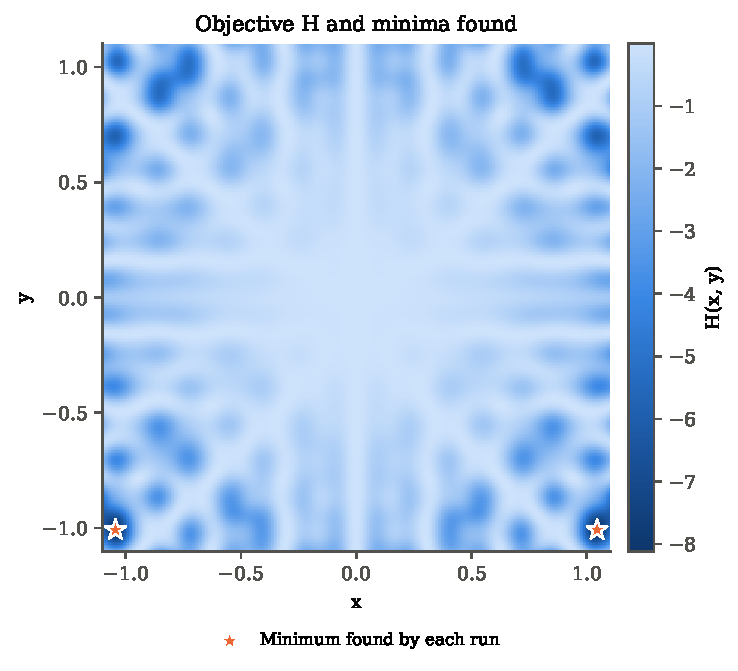
\includegraphics[width=0.6\textwidth]{q1_annealing.pdf}
\end{center}

\newpage
\section*{Q2. Simulated annealing for 100-city tours}

I interpreted the requested average as an average over independently generated city sets. I generated 20 sets,
each containing 100 cities sampled uniformly from $[0, 100] \times [0, 100]$ miles, and ran annealing once on
each set from a random tour.

A tour is an ordering of all 100 cities. Its length is the sum of Euclidean distances between consecutive
cities, including the return from the last city to the first. Each proposal reverses one segment of the tour
(a 2-opt move). It therefore keeps every city exactly once. The acceptance rule is the Q1 rule with tour
length in place of $H$.

\begin{center}
\begin{tabular}{p{0.45\textwidth}p{0.45\textwidth}}
\toprule
\textbf{Setting / result} & \textbf{Value} \\
\midrule
City sets / seed & 20 / 546 \\
Cooling schedule & Geometric, from $T = 10$ to $T = 0.05$ \\
Proposed moves per run & 500,000 \\
\textbf{Average shortest tour across 20 sets} & \textbf{800.4 miles} \\
\bottomrule
\end{tabular}
\end{center}

These are the shortest tours found within the stated budget. Their true optimality is not certified, so the
average may be slightly above the average of the exact shortest tours.

\begin{center}
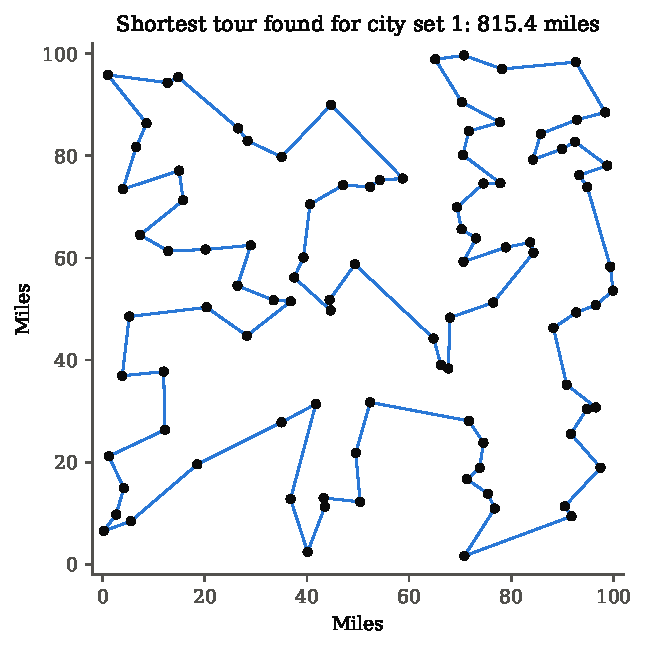
\includegraphics[width=0.55\textwidth]{q2_tsp.pdf}
\end{center}

\newpage
\section*{Q3. Simulated tempering for the witch's hat}

The state is a vector of 30 numbers between 0 and 1. Let $B = [0, 1/3]^{30}$ be the narrow hat region, and let
$a = (3^{30} - 1)/2$. The unnormalized density $g(x)$ equals $a$ inside $B$ and 1 outside. The hat volume is
$v = 3^{-30}$, about $4.86 \times 10^{-15}$. The exact probability of the hat is $va / (va + 1 - v) = 1/3$,
which gives a direct check on the simulation.

For this two-level density the normalizing constants can be calculated directly. With $\beta$ denoting inverse
temperature, I used
\[
\pi_\beta(x) = \frac{g(x)^\beta}{Z_\beta}, \qquad Z_\beta = (1 - v) + v a^\beta .
\]
The 20 inverse temperatures are $\beta = 0.05, 0.10, \ldots, 1$, and $\beta = 1$ is the requested target. I used
weights $1/Z_\beta$, so each temperature has the same probability in the joint distribution.

\subsection*{One iteration}

\textbf{Position update.} With equal probability, propose uniformly from the whole cube or uniformly from the
hat. This gives the proposal density $q(x) = 0.5 + 0.5/v$ inside $B$ and $q(x) = 0.5$ outside $B$. The MH
correction is
\[
\alpha_x = \min\left\{1, \frac{g(y)^\beta q(x)}{g(x)^\beta q(y)}\right\}.
\]
A proposal from the whole cube alone would almost never enter the hat, because the hat is so small.

\textbf{Temperature update.} Propose one index higher or lower with equal probability. An attempt to move
beyond the ladder is rejected. For a valid proposed inverse temperature $\beta'$, accept with
\[
\alpha_\beta = \min\left\{1, \frac{g(x)^{\beta'} Z_\beta}{g(x)^{\beta} Z_{\beta'}}\right\}.
\]

\begin{center}
\begin{tabular}{p{0.45\textwidth}p{0.45\textwidth}}
\toprule
\textbf{Setting / result} & \textbf{Value} \\
\midrule
Iterations / discarded / seed & 1,100,000 / 100,000 / 546 \\
Samples at $\beta = 1$ (every 4th state) & 12,360 \\
\textbf{Probability of being in the hat} & \textbf{0.336 (exact 1/3)} \\
\bottomrule
\end{tabular}
\end{center}

\begin{center}
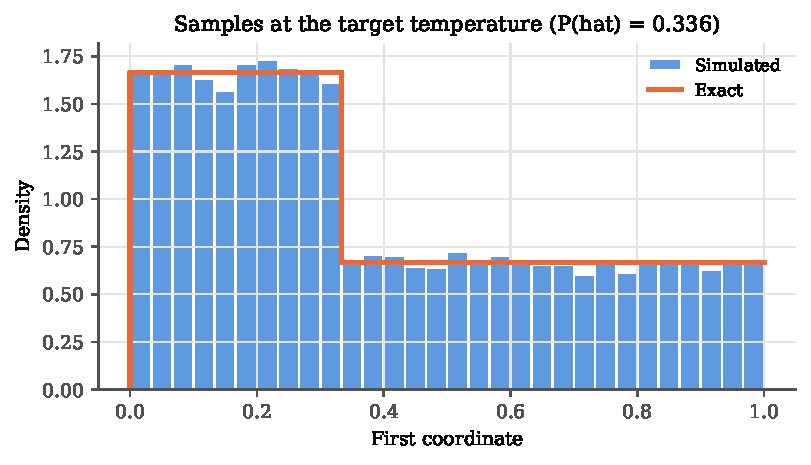
\includegraphics[width=0.65\textwidth]{q3_witch_hat.pdf}
\end{center}

\newpage
\section*{Q4. Double MH for the very-soft-core model}

\subsection*{Data and prior used for the numerical example}

The assignment does not supply a point pattern, $n$, or the region $A$. I used $n = 50$ points in the unit
square $A = [0, 1]^2$. The observations were simulated at $\theta = 1$ using 500 sweeps of point updates,
starting from uniform points. The coordinates are saved with the results.

\textbf{Prior assumption:} I used $p(\theta) \propto 1/\theta$ on $0.001 \le \theta \le 10$. A finite range is
needed here: as $\theta$ approaches zero or infinity, the likelihood approaches a positive constant, so
multiplying by $1/\theta$ gives an infinite integral. The unrestricted prior in the question does not produce a
proper posterior for this model. The finite bounds are an explicit extra assumption.

\subsection*{Updates}

Write $U(x, \theta)$ for the sum of pairwise potentials in the question, so the likelihood is
$\exp[-U(x, \theta)]/Z(\theta)$. I update $\eta = \log(\theta)$ with a normal random walk of standard
deviation 0.6. Proposals outside the prior range are rejected.

For each proposed $\theta'$, initialize an auxiliary point pattern $y$ at the observed pattern and run one
sweep at $\theta'$: 50 updates, each moving a randomly chosen point to a uniform location in the square and
accepting with $\min\{1, \exp[-\text{change in } U]\}$. The outer acceptance probability is then
$\min(1, \exp(\log r))$, with
\[
\log r = U(x, \theta) - U(x, \theta') + U(y, \theta') - U(y, \theta).
\]
The normalizing constants cancel in this ratio. The $1/\theta$ prior and the correction for proposing on the
log scale also cancel inside the prior bounds.

\begin{center}
\begin{tabular}{p{0.45\textwidth}p{0.45\textwidth}}
\toprule
\textbf{Setting / result} & \textbf{Value} \\
\midrule
Outer iterations / discarded / seed & 11,000 / 1,000 / 546 \\
Inner simulation & 1 sweep = 50 proposed point updates \\
Outer acceptance & 50.9\% \\
\textbf{Posterior mean} & \textbf{1.205} \\
\textbf{95\% posterior interval} & \textbf{[0.380, 2.376]} \\
\bottomrule
\end{tabular}
\end{center}

The generating value $\theta = 1$ is inside the posterior interval.

\begin{center}
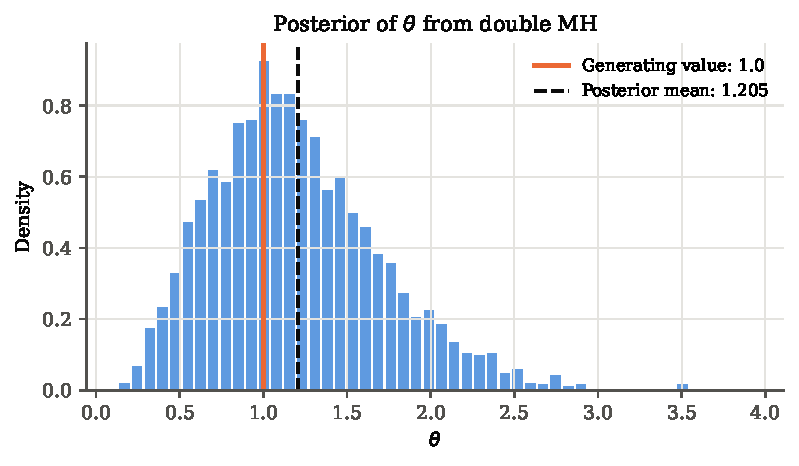
\includegraphics[width=0.55\textwidth]{q4_soft_core.pdf}
\end{center}

\end{document}
